\documentclass{article}
\usepackage[utf8]{inputenc}
%\usepackage{natbib}
\usepackage{graphicx}
\usepackage[hidelinks]{hyperref}
\usepackage{color}
\usepackage{listings}
%\usepackage{lastpage}
%\usepackage{wrapfig}
%\usepackage{eso-pic}
%\usepackage{tikz}
\usepackage{float}
\usepackage{amssymb}
\usepackage{caption}
\usepackage{subcaption}
%\usepackage{pdfpages}
\usepackage[backend=biber]{biblatex}
\definecolor{commentgreen}{RGB}{100, 190, 100}
\definecolor{gray}{RGB}{50, 50, 50}
\lstset{language=C,
                breaklines=true,
                basicstyle=\ttfamily\scriptsize,
                keywordstyle=\color{blue}\ttfamily,
                stringstyle=\color{red}\ttfamily,
                commentstyle=\color{commentgreen}\ttfamily,
                morecomment=[l][\color{magenta}]{\#},
                numberstyle=\tiny\color{gray},
                numbers=left
}


\title{RAT - Mini-project:}
\author{Jannick Drews}
\date{\today}

\newcommand{\secref}[1]{\nameref{#1}~\ref{#1}}
\newcommand{\goodcite}[1]{\textsuperscript{\cite{#1}}}

\addbibresource{Ref.bib}

\setlength\parindent{0pt}
\begin{document}
\pagenumbering{gobble}
\maketitle
\newpage
\pagenumbering{arabic}

%% For this mini-project, you have to create and showcase an advanced shader and talk about the theory behind it.
%% You should be able to depict a deep understanding of your code, to be able to explain how it works and how you
%%  overcome the technical challenges you met.  Such shader can be, but not limited to: %% list of suggestions here%%
%%
\begin{figure}[H]
	\centering
	%\includegraphics[width=\textwidth]{img/animation_setup.png}
	\caption{Setup of animation}
	\label{fig:animation_setup}
\end{figure}

\section{Composite}
\begin{figure}[H]
	\centering
	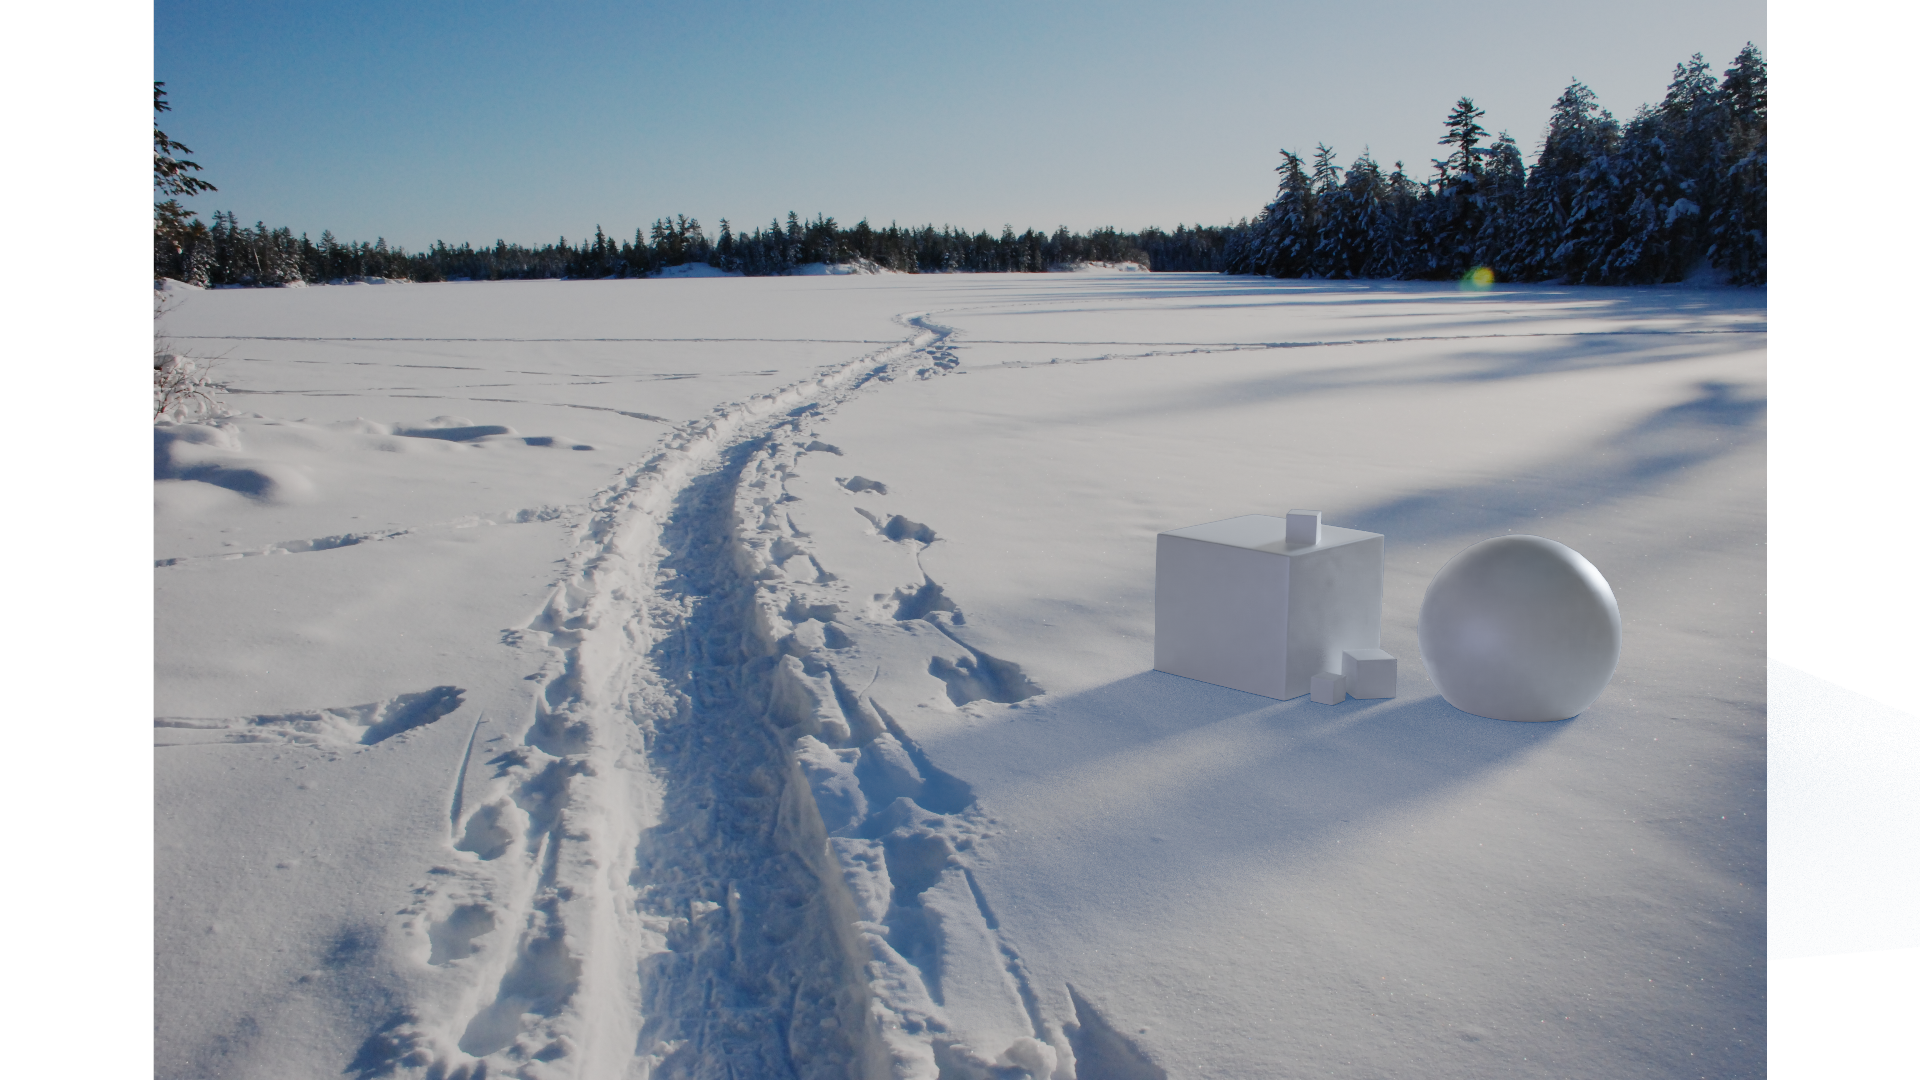
\includegraphics[width=\textwidth]{img/RAT.png}
	\caption{Final render}
	\label{fig:final_render}
\end{figure}

\begin{figure}[H]
	\centering
	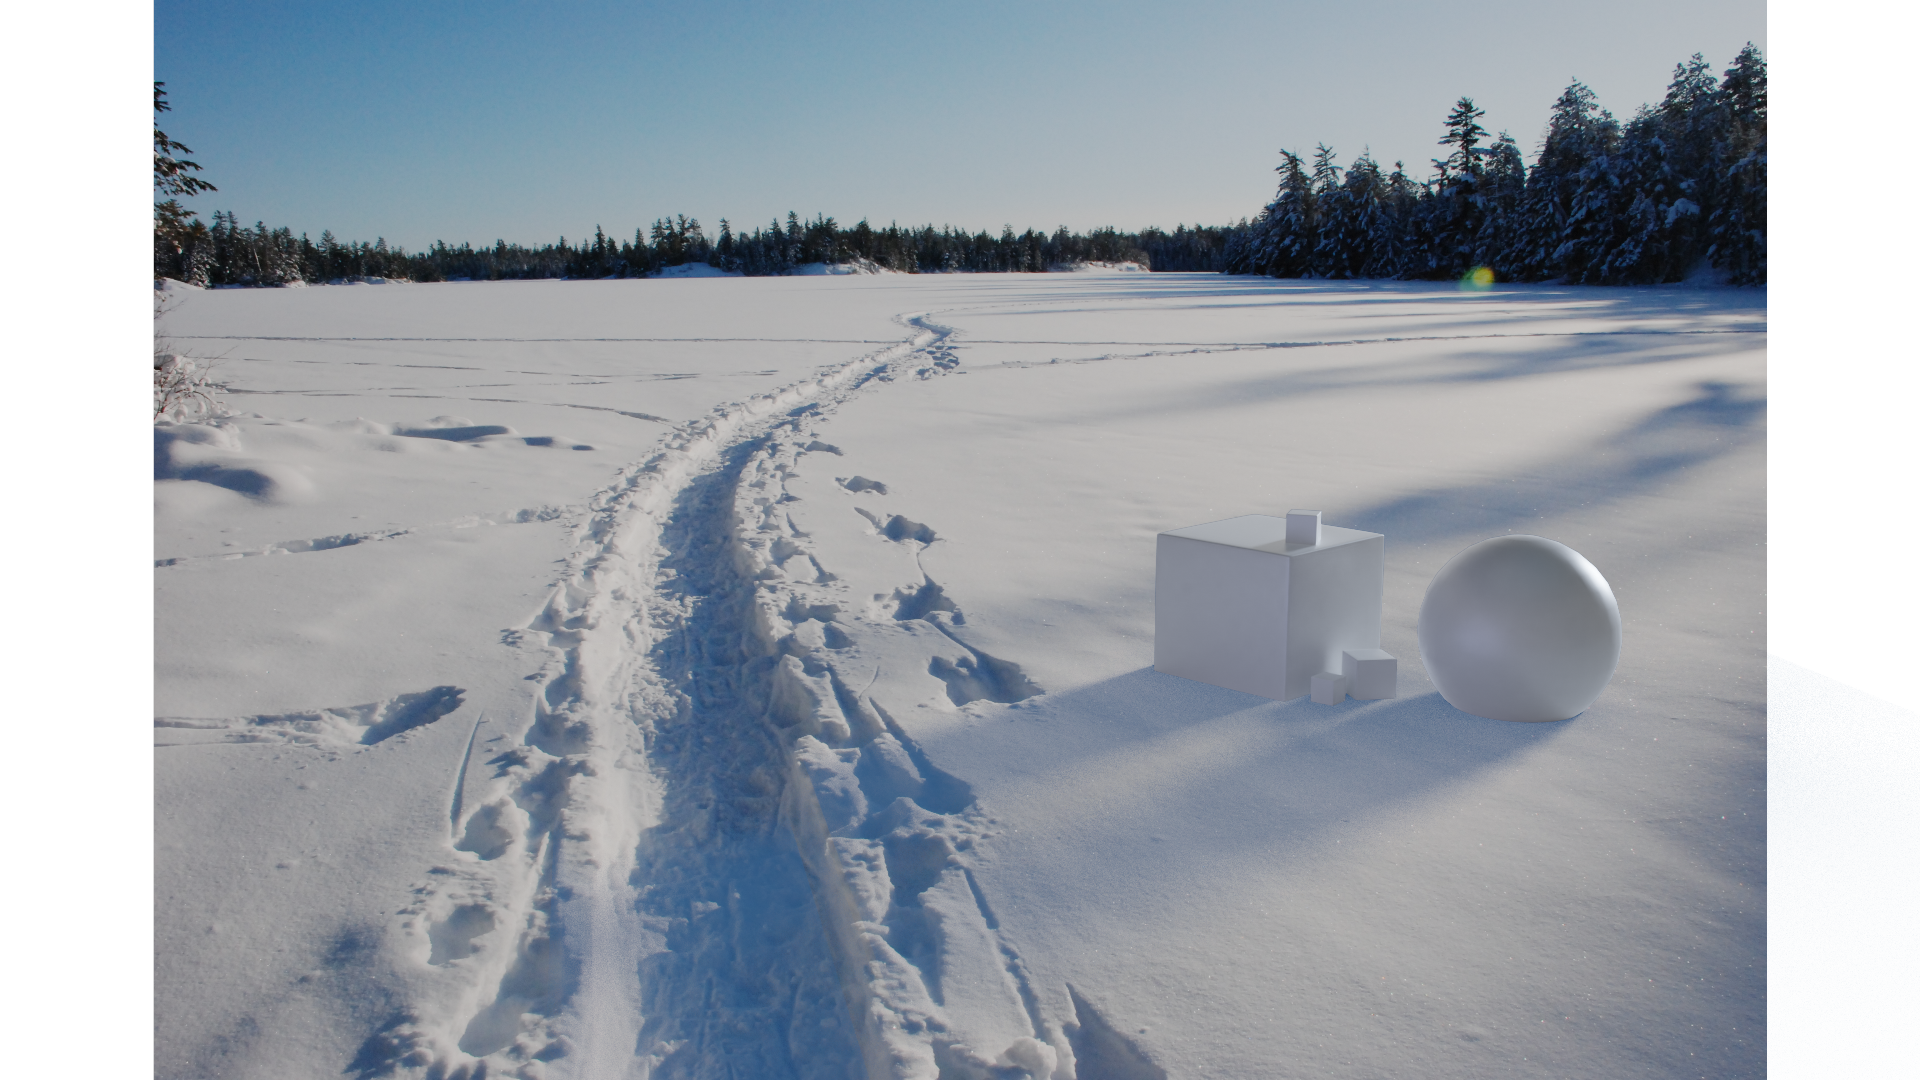
\includegraphics[width=\textwidth]{img/tried_to_fix.png}
	\caption{Final render}
	\label{fig:final_render}
\end{figure}

\begin{figure}[H]
	\centering
	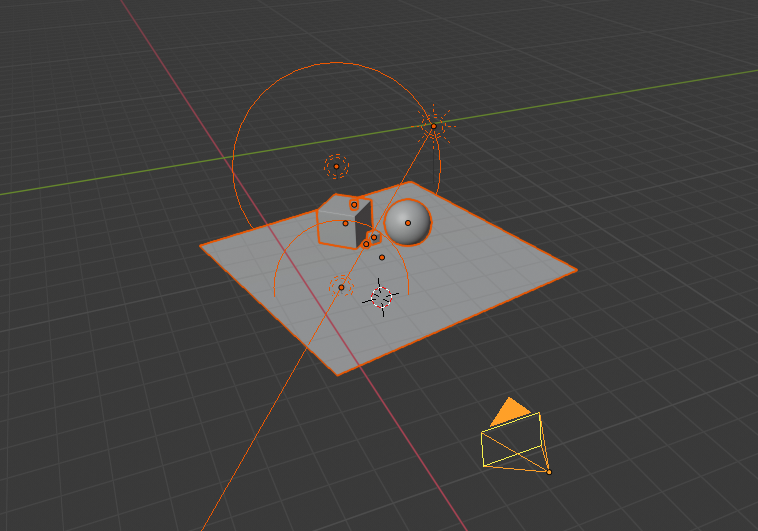
\includegraphics[width=\textwidth]{img/scene_setup.png}
	\caption{Setup of scene}
	\label{fig:scene_setup}
\end{figure}

\begin{figure}[H]
	\centering
	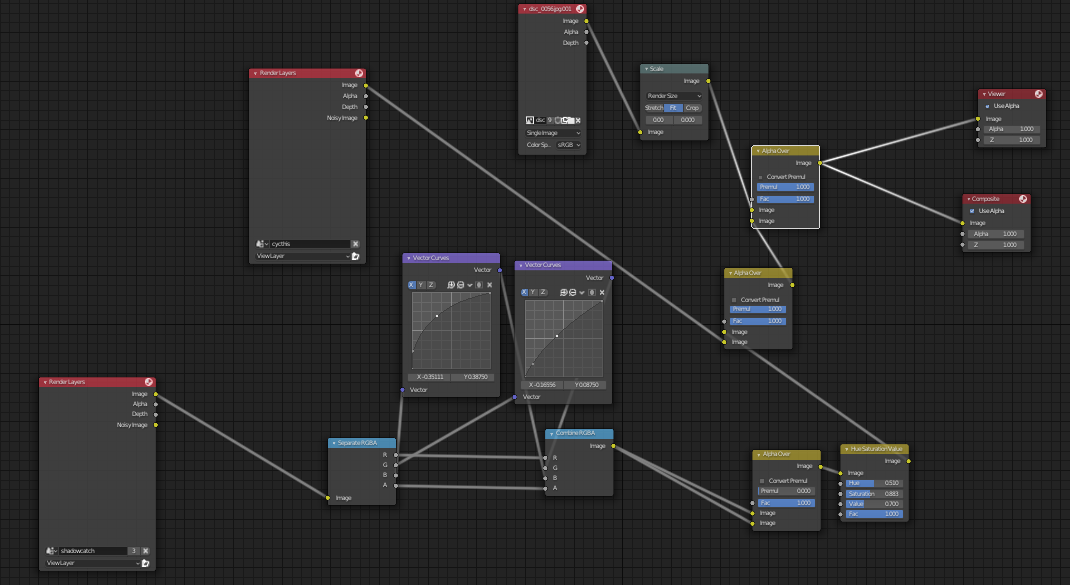
\includegraphics[width=\textwidth]{img/node_setup.png}
	\caption{Setup of nodesystem}
	\label{fig:node_setup}
\end{figure}

\begin{figure}[H]
	\centering
	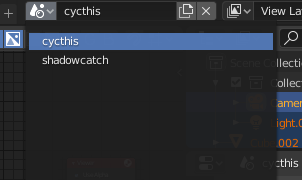
\includegraphics[width=\textwidth]{img/layer_setup.png}
	\caption{Setup of layers}
	\label{fig:shadow_setup}
\end{figure}


%\newpage
\section{Bibliography}
\printbibliography


\end{document}

